\documentclass[12pt]{article}
\usepackage{graphics}
\usepackage{amsmath}
\usepackage{mathtools}
\usepackage{gensymb}

\newcommand{\mydet}[1]{\ensuremath{\begin{vmatrix}#1\end{vmatrix}}}
\providecommand{\brak}[1]{\ensuremath{\left(#1\right)}}
\providecommand{\norm}[1]{\left\lVert#1\right\rVert}
\newcommand{\solution}{\noindent \textbf{Solution: }}
\newcommand{\myvec}[1]{\ensuremath{\begin{pmatrix}#1\end{pmatrix}}}
\let\vec\mathbf

\begin{document}
\begin{center}
\textbf\large{CHAPTER-7 \\ COORDINATE GEOMETRY}

\end{center}
\section*{Excercise 7.1.}

Q8.Find the Value of y for which the distance between the points P(2,-3) and Q(10,y) is 10 units:
\begin{enumerate}
	\item $\brak{2,-3,}, \brak{10,y}$ 
\end{enumerate}
\solution
\begin{enumerate}
\item The coordinates are given as
	\begin{align}
	\vec{P} = \myvec{
		2\\
	   -3\\
		},
	\vec{Q} = \myvec{
	   10\\
		y\\
		},
	\end{align}
	\begin{align}
		\vec{P} - \vec{Q} = \myvec{2\\-3} - \myvec{10\\y} = \myvec{-8\\-3-y}\\		
	\end{align}
	
	
	
	
	\begin{align}
			(\vec{P}-\vec{Q})^\top (\vec{P}-\vec{Q}) = \myvec{-8&-3-y} \myvec{-8\\-3-y} = y^2+6y+9+64
	\end{align}
	
	
	\begin{align}
	d={\norm{\vec{P}-\vec{Q}}}=\sqrt{\brak{\vec{P} -\vec{Q}}^{\top}\brak{\vec{P} -\vec{Q}}}
	\end{align}
	
	\begin{align}
	Given, d=10 units, therefore \\
	10 = \sqrt{y^2+6y+9+64}
	\end{align}
	
	\begin{align}
		Removing\:root\:on\:Right\:Hand\:Side(RHS) \\
			100 = y^2 + 6y + 73 \\
				y^2 + 6y + 73 - 100 = 0 \\
					y^2 + 6y - 27 = 0 \\
						(y-3)(y+9) = 0 \\
	\end{align}
	
    Hence, the values of y for given point P(2,-3) and Q(10,y) is " y = 3 or y = -9".	
\hspace{3mm}
\begin{figure}[!h]
	\begin{center}
	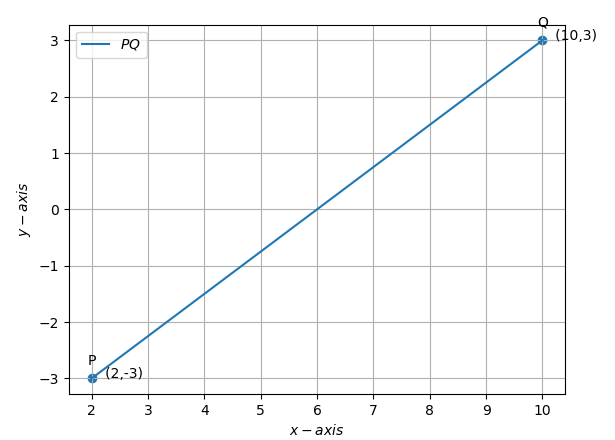
\includegraphics[width=6in]{graph.png}	
	\end{center}
		
\caption{Graph for the line}
\label{fig:Fig}
\end{figure}
\end{enumerate}
\end{document}
	
